\section{Scaling up the Number of Processes}
\label{sec:n_nodes}

The previously discussed master-worker algorithm expects all input tensors before and the output tensor after a contraction to reside within a single master process.
Imagine we now have $p$ processes.
The master process is now involved in sending and receiving $\frac{p-1}{p}$ parts of the tensors in the contraction.
Meanwhile, the worker processes each only communicate $\frac{1}{p}$ parts of the tensors with the master.
The larger $p$ gets the more unbalanced communication in the master-worker algorithm gets.
It also might run into memory issues should the total size of all tensors exceed the master process' memory size.

Instead, let us consider algorithms that work on distributed tensors as input and output.
Such algorithms allow the communication load to be balanced across all processes.

As basis for such an algorithm, we make the following assumptions:
\begin{enumerate}
    \item input tensors are predistributed across all processes
    \item output tensors may stay distributed
    \item tensors are sufficiently compute intensive that communication is not a bottleneck
    \item the distributed dimension is a multiple of the total number of processes $p$
    \item each process has multiple threads.
\end{enumerate}

% todo: justify assumptions after talking about algorithms

Given sufficiently large einsum trees with sufficiently large tensors the initial predistribution of the input tensors and the final gather of the output tensor will consume a negligible amount of time compared to the evaluation of the tree.
They will also generally have a higher compute intensity enabling a high throughput despite the lower network speed compared to local memory speeds.
These assumptions indicate that the proposed algorithms need a minimum tensor size to show improvements over the base \texttt{einsum\_ir} implementation.

Assumption 4 is merely necessary to simplify the algorithms worked on for this paper.
Should assumption 4 not hold true, for example if a dimension $o$ with $|o|=14$ gets split across $p=4$ processes, the data could be distributed as $4 4 3 3$ or $4 4 4 2$.
In either case each communication and contraction would merely need at most four variants depending on both input tensor states, either having a "full" chunk with $|o'|=4$ or a "partial" chunk with either $|o''|=3$ or $|o''|=2$.
The last assumption is needed as some of the following algorithms use an extra communication thread.
This thread is solely responsible for pushing all communication and feeding the computation threads continuously with data to process.
This design was chosen as to overlap communication with computation to minimize waiting times due to network speeds.

With those assumptions we will conceive three algorithms:

\subsection{Distributed c Dimension}

\begin{figure}[ht]
    \centering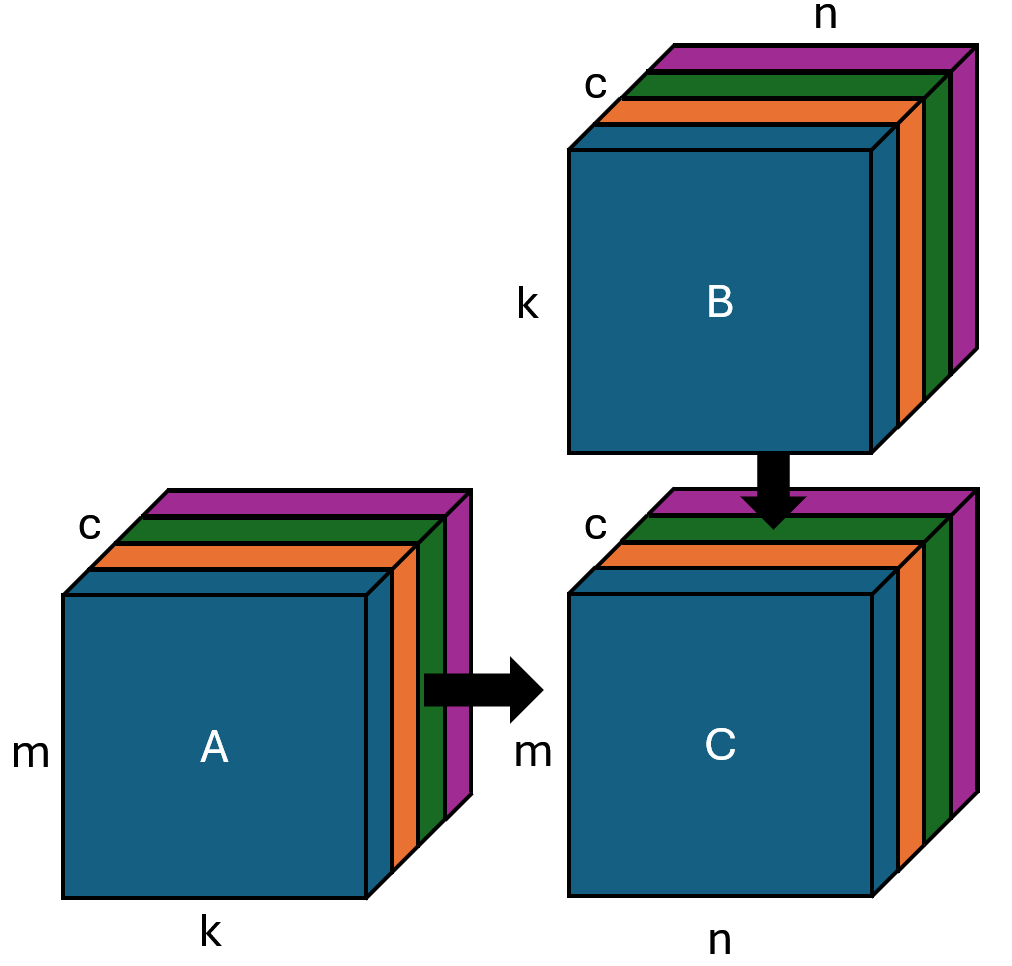
\includegraphics[width=0.3\textwidth]{dist_c.png} 
    \caption{Visualization of the distributed c algorithm for the contraction $cmk,ckn \rightarrow cmn$; 
    each color represents a process and the data they hold; 
    since the tensors are distributed along the same c dimension, each node can locally contract its chunks to generate its chunk of the output tensor.}
    \label{fig:c_algo}
    \end{figure}

\begin{algorithm}[ht]
    \begin{algorithmic}
    \Require $i = \texttt{mpi\_rank}, A_i, B_i$
    \Ensure $C_i$
    \State $A_i, B_i \rightarrow C_i$
\end{algorithmic}
\caption{Distributed c contraction}
\label{alg:c_pseudocode}
\end{algorithm}

Imagine $A$,$B$ and $C$ are distributed over a c dimension $c_0$.
As described in \ref{sec:einsum_expr} in such a case each process has to only contract its local chunks.
This algorithm is the best case since no communication has to occur and cutting a tensor among its c dimension keeps its compute intensity.

\subsection{Distributed m and n Dimensions}

\begin{algorithm}[ht]
        \begin{algorithmic}
        \Require $i = \texttt{mpi\_rank}, A_i, B_i$
        \Ensure $C_i$
        \State $\texttt{next} = (i+1) \mod p$
        \State $\texttt{prev} = (i+p-1) \mod p$
        \State $\texttt{comp\_buffer} \gets B_i$
        \State  $\text{for } j \text{ in } 0\dots p - 1 \text{ do:}$
        \State \indent $k \gets (i + j) \mod p$
        \State \indent \text{do in parallel:}
        \State \indent \indent $A_i, \texttt{comp\_buffer} \rightarrow C_{i,j}$
        \State \indent \indent $\texttt{mpi\_recv recv\_buffer from next}$
        \State \indent \indent $\texttt{mpi\_send comp\_buffer to prev}$
        \State \indent $\texttt{comp\_buffer} \gets \texttt{recv\_buffer}$
        \State $C_i \gets \texttt{concat}(C_{i,0}\dots C_{i,p})$
    \end{algorithmic}
    \caption{Distributed m/n contraction}
    \label{alg:m_n_pseudocode}
\end{algorithm}

%todo: reword algorithm (?) and double check which variant I am describing in text (m_n_out_n or m_n_out_m)

Imagine $A$ and $C$ share an m dimension $m_0$ and $B$ and $C$ share an n dimension $n_0$.
Contracting an expression $A,B \rightarrow C$ is then the same as splitting $A$ along $m_0$ into $p$ chunks $A_0\dots A_{p-1}$ and $B$ along $n_0$ into $p$ chunks $B_0\dots B_{p-1}$.
We can imagine $C$ then as the concatenation of $C_0\dots C_p$ chunks split along the $m_0$ dimension and $C_i$ for $0 \leq i \leq p$ as the concatenation of $C_{i,0} \dots C_{i,p}$ along $n_0$.
We can compute each $C_{i,j}$ as $A_i,B_j \rightarrow C_{i,j}$.
To calculate a chunk $C_i$ a process needs all of $A$.
Instead of executing an \texttt{allgather} on $A$ we will calculate $C_i$ stepwise.
In each step each process will contract one part $C_{i,j}$ of $C_i$ as $A_i,B_j \rightarrow C_{i,j}$.
Simultaneously each process will get a new chunk $B_{j+1}$ from their neighbour with a higher rank in a ring, so the process with the highest rank gets its chunk from the process with rank 0.
To enable both the contraction and the communication of the new chunk to occur simultaneously each process needs extra memory with the size of one chunk of $B$ and employ an extra communication thread to fulfill the communication on that extra chunk.
Since we assume all tensors to be predistributed, each process will begin with its diagonal part $C_{i,i}$ where i equals the rank of the process.
Following the above algorithm each process will compute $C_{i,i}, \dots C_{i,p-1},C_{i,0},\dots,C_{i,i-1}$.
After we concatenate those chunks $C_{0,i}\dots C_{p-1,i}$ to $C_i$ our algorithm is done and $C$ is distributed along $n_0$.

In the implementation we can make the final concatenation implicit as long as we contract each chunk $C_{i,j}$ already with the correct strides into the output tensor $C_i$.
Due to limitations in the binary contraction described in Section \ref{sec:einsum_ir} this is only possibly should each chunk $C_{i,j}$ be contiguous in $C_i$.
To fulfill that the implementation has to restrict the $m_0$ dimension to be the outermost dimension of $C$.

We could also consider another very similar algorithm where each process gets a chunk $A_i$ in each step instead of $B_j$.
Such an algorithm is omitted here, since the same effect can be achieved by swapping the input tensors as $A' \coloneqq B$ and $B' \coloneqq A$, which results in $A',B' \rightarrow C$.

The algorithm employs a ring-like communication pattern to reduce memory usage.
Instead of moving all the tensors in each time step, one could imagine an algorithm where each process keeps its chunk $B_i$ and sends them directly to whichever process that needs it.
That comes with the problem of still needing one tensor to contract on and another to handle the communication at the same time.
Since the initial tensor $B_i$ may no longer be moved now, this takes an additional buffer of size $|B_i|$.

\subsection{Distributed k Dimension}


\begin{algorithm}[ht]
    \begin{algorithmic}
        \Require $\texttt{send\_buffer},\texttt{comp\_buffer},\texttt{recv\_buffer}$
        \Ensure $\texttt{send\_buffer},\texttt{comp\_buffer},\texttt{recv\_buffer}$
        \State $\texttt{temp} \gets {send\_buffer}$
        \State $\texttt{send\_buffer} \gets {comp\_buffer}$
        \State $\texttt{comp\_buffer} \gets {recv\_buffer}$
        \State $\texttt{recv\_buffer} \gets {temp}$
    \end{algorithmic}
    \caption{rotate}
    \label{rotate_pseudocode}
\end{algorithm}

\begin{algorithm}[ht]
    \begin{algorithmic}
    \Require $i = \texttt{mpi\_rank}, A_i, B_i, j$
    \Ensure $C_i$
    \State $\texttt{next} = (i+1) \mod p$
    \State $\texttt{prev} = (i+p-1) \mod p$
    \State $\texttt{send\_buffer} \gets \texttt{firstHalf}(C_i)$
    \State $\texttt{comp\_buffer} \gets \texttt{secondHalf}(C_i)$
    \State $\texttt{recv\_buffer} \gets \texttt{new memory}$
    \State $\text{repeat } (p+1) \mod 3 \text{ times} \texttt{ //last contraction on secondHalf}(C_i)$ 
    \State \indent $\texttt{rotate}(\texttt{send\_buffer},\texttt{comp\_buffer},\texttt{recv\_buffer})$
    \State $A_{i,0}, B_{i,next} \texttt{comp\_buffer}$
    \State  $\text{for } j \text{ in } 0\dots 2 * p - 1 \text{ do:}$
    \State \indent $ k = j \mod 2 $
    \State \indent $ m = (i + 1 + \frac{j}{2}) \mod p$
    \State \indent \text{do in parallel:}
    \State \indent \indent $A_{i,k}, B_{i,m} \rightarrow \texttt{comp\_buffer}$
    \State \indent \indent $\texttt{mpi\_recv recv\_buffer from next}$
    \State \indent \indent $\texttt{mpi\_send send\_buffer to prev}$
    \State \indent $\texttt{rotate}(\texttt{send\_buffer},\texttt{comp\_buffer},\texttt{recv\_buffer})$
    \State $A_{i,1}, B_{i,i} \rightarrow \texttt{comp\_buffer}$

\end{algorithmic}
\caption{Distributed k contraction}
\label{alg:k_pseudocode}
\end{algorithm}

If a tensor contraction $A,B \rightarrow C$ shares a dimension between both input tensor, but not in the output tensor, we will call it a k dimension.
Imagine $A$ and $B$ share a k dimension $k_0$.
Contracting an expression $A,B \rightarrow C$ is the same as splitting $A$ and $B$ along $k_0$ into p chunks $A_0\dots A_{p-1}$ and $B_0\dots B_{p-1}$.
If we define $C_i$ as the result from $A_i,B_i \rightarrow C_i$, $C=\sum{C_i}$.
To receive a distributed output tensor we would have to split $C$ into $p$ chunks $C_0\dots C_{p-1}$ again.
Instead of first computing the whole of C on each process, we can compute partial sums of the output tensors $C_j$, where 
$C_j = \sum_{i=0}^{p-1} C_{i,j}$.
Each process $j$ can compute all updates $C_{0,j}\dots C_{p-1,j}$.
To end each process on its chunk $C_j$ we imagine each process adding its partial sum $C_{i,j}$ to an existing partial sum of $C_i$ and then communicating this partial sum to its previous neighbour $j+p-1 \mod p$.
If each process starts adding upon $C_{j+1}$, it will end up with $C_j$ after all processes have added all partial sums to $C_j$.
This $C_j$ may be split across any arbitrary dimension.

If we want to overlap communication and computation in an implementation we have to slightly adjust the algorithm.
If we compute partial updates on all of $C_j$ each process has to wait communicating the partial updates until the computation is done.
Instead, each process should compute half of $C_j$ and already communicate that part while it computes the second half of the partial updates upon it.
Doing this we can continuously contract on each process.